\documentclass{deliverablereport}

\usepackage[style=alphabetic,backend=bibtex]{biblatex}
\addbibresource{../../lib/kbibs/kwarcpubs.bib}
\addbibresource{../../lib/kbibs/extpubs.bib}
\addbibresource{../../lib/kbibs/kwarccrossrefs.bib}
\addbibresource{../../lib/kbibs/extcrossrefs.bib}
\addbibresource{../../lib/deliverables.bib}
%\addbibresource{../../lib/publications.bib}
\addbibresource{rest.bib}
% temporary fix due to http://tex.stackexchange.com/questions/311426/bibliography-error-use-of-blxbblverbaddi-doesnt-match-its-definition-ve
\makeatletter\def\blx@maxline{77}\makeatother

\deliverable{hpc}{pythran-sage}
\deliverydate{02/27/2017}
\duedate{02/27/2017 (Month 18)}
\def\pn{OpenDreamKit}
\author{}

\begin{document}
\maketitle
%  Work Package WP6 develops a novel, foundational, knowledge-based framework for
  interfacing existing open source mathematical software systems and knowledge bases into
  a mathematical VRE, where systems can delegate functionalities among each other
  seamlessly without losing semantics.

  The overall Math-in-the-Middle (MitM) Framework developed in WP6 over the last three
  years is described in D6.5; this Report complements it by describing the curated
  contents Math-in-the-Middle (MitM) Ontology which serves as a reference and pivotal
  point for translations between the various input languages of mathematical software
  systems and knowledge bases.

  In a nutshell, the MitM Ontology describes the mathematical objects, concepts, and their
  relations in a general, system-agnostic way in an OMDoc/MMT theory graph while the
  mathematical systems export API theories that describe the system interface language in
  terms of types, classes, constructors, and functions -- again in OMDoc/MMT. These two
  levels of descriptions are linked by OMDoc/MMT alignments that allow the translation of
  expressions between systems.

%%% Local Variables:
%%% mode: visual-line
%%% fill-column: 5000
%%% mode: latex 
%%% TeX-master: "report"
%%% End:

\strut\githubissuedescription
\newpage\tableofcontents\newpage

\section{Introduction}

The aim of this project is to optimize the overall performance of Cython code
that uses Numpy arrays.

Indeed, when operations are done on Numpy arrays, Cython relies on the original
Numpy package to compute them. This involves a fall back to the Python
interpreter. It thus misses several optimisation opportunities, especially with
complex expressions.

The Pythran project is a Python to C++ compiler, that aims at optimizing
scientific Python. It thus supports only a subset of the Python language.
It also has a full C++ implementation of a major set of the Numpy API. Some of
the advantage of this implementation is that it supports expression templates
and SIMD instructions. Expression templates allow to "fuse" loops that can
occurs when expressions with multiple operators are computed. For instance,
the expression $a+b*c$ will original be transformed by Cython in two call: one
for the multiplication of $b$ by $c$, and one for the addition of the result of
this multiplication and the addition by $a$. Each call will end-up in one loop,
that will read memory, compute the operation and write back to memory. The
second loop will have the same pattern. In nowadays architecture, memory
bandwidth is often the limiting factor in this kind of operation. It is thus
really interesting to merge these loops, and load/store the memory only once.
Expression templating is a C++ technique that allows to evaluate expressions
only when they are stored to memory. Thus, in this case, the two loops will be
automatically "merged" by the C++ compiler, and we'll get an optimized version
of this code. Note that this technique is used for instance by the C++ wrapper
of the GMP library.

\section{Cython and Pythran integration}

The project has been focused on using this Pythran backend for numpy arrays in
Cython when possible. Indeed, Pythran has a few limitations regarding the numpy
arrays it can handle:

\begin{itemize}
  \item array "views" are not supported. That means that arrays must be stored
    in conitguous memory. Fortran and C-style format are supported.
  \item the endianess of the integers must be the same that the one of the
    targeted architecture (note that Cython has the same limitation)
\end{itemize}

We thus need to be able to fall-back to the Cython implementation if we are not
in one of those cases.

The integration within Cython works this way:

\begin{itemize}
  \item at the function level, for every argument that is an numpy array and
    supported by Pythran, we change its type by a fused type
    \footnote{\url{http://cython.readthedocs.io/en/latest/src/userguide/fusedtypes.html}}.
    This fused type is whether a Pythran numpy buffer or the original Cython
    buffer type
  \item for variable defined as numpy array, we change them directly to a
    Pythran buffer, if their type and endianess are supported.
\end{itemize}

Cython has a comprehensive suite test regarding the Numpy features it supports.
This test suite is still valid after this integration.

\section{Usage}

A new flag {\tt --np-pythran} has been added to Cython that enables the usage
of Pythran for Numpy operations. It will generate a C++ file that uses the
optimized Numpy functions that are in Pythran.

Then, when compiling the final extension, a path to an existing Pythran
installation must be provided.

Here is an example of usage using {\tt distutils}:

More detailed example are provided in the documentation (within the Cython PR,
see section~\ref{sec:links}).

\section{Benchmarks}

We did some benchmarks to see the benefits of the Pythran integration for Numpy
operations. These benchmarks have been done using an Intel Core i7-6700HQ.

\subsection{Float computation}

Here is a code snippet that does some computation on floating-point values:

\begin{lstlisting}[language=python]
import numpy
cimport numpy
def float_comp(numpy.ndarray[numpy.float_t, ndim=1] a, \
             numpy.ndarray[numpy.float_t, ndim=1] b):
    return numpy.sqrt(numpy.sqrt(a*a+b*b))
\end{lstlisting}

The figure~\ref{fig:float_bench} shows the compute time for various sizes for
{\tt a} and {\tt b}, using the original Cython mode, then Cython with the
Pythran backend, and finally Cython with the Pythran backend and SIMD
instructions.

\begin{figure}[h]
  \caption{\label{fig:float_bench} Float computation benchmark (logarithmic scales)}
  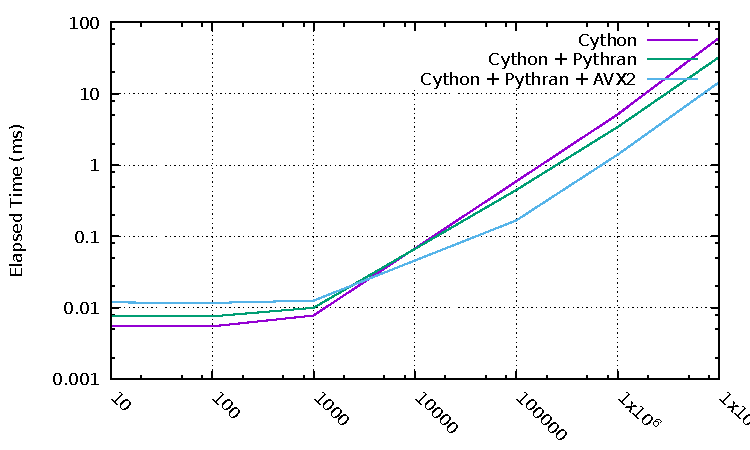
\includegraphics{benchs/float/graph.pdf}
\end{figure}

\subsection{Convolution}

We used this example from the Cython documentation:
\url{http://cython.readthedocs.io/en/latest/src/tutorial/numpy.html}.

The input we use is the following:

\begin{lstlisting}[language=python]
import numpy as np
N = 1000
f = np.arange(N*N, dtype=np.int).reshape((N,N))
g = np.arange(81, dtype=np.int).reshape((9, 9))
\end{lstlisting}

The results are the following:

\begin{itemize}
  \item for the classical Cython version: 155ms
  \item for the Cython version using the Pythran backend: 150ms
  \item for the Cython version using the Pythran backend using SIMD instructions: 149ms
\end{itemize}

It seems the Pythran backend don't manage to benefit a lot from SIMD
instructions in this case. We thus still got an average speedup of ~3 \%.

\section{Links}
\label{sec:links}

Modifications that were necessary to the Pythran project have been accepted and
merged into its master branch (see
\url{https://github.com/serge-sans-paille/pythran/pull/629},
\url{https://github.com/serge-sans-paille/pythran/pull/628},
\url{https://github.com/serge-sans-paille/pythran/pull/616} and
\url{https://github.com/serge-sans-paille/pythran/pull/614}).

The modifications necessary within the Cython project are currently reviewed
(see \url{https://github.com/cython/cython/pull/1607}).

\printbibliography
\end{document}

%%% Local Variables:
%%% mode: latex
%%% TeX-master: t
%%% End:

%  LocalWords:  githubissuedescription newpage tableofcontents newpage printbibliography
